%%%%%%%%%%%%%%%%%%%%%%%%%%%%%%% beamer %%%%%%%%%%%%%%%%%%%%%%%%%%%%%%%%%%%%%%%%%%%%%%%%%
% To run - pdflatex filename.tex
%	   acroread filename.pdf
%%%%%%%%%%%%%%%%%%%%%%%%%%%%%%%%%%%%%%%%%%%%%%%%%%%%%%%%%%%%%%%%%%%%%%%%%%%%%%%%%%%%%%%%
%\documentclass[handout,compress,gray]{beamer}
\RequirePackage{flashmovie}
\documentclass[utf8x,compress,black]{beamer} 
\mode<presentation>
\usetheme{Madrid}

\hypersetup{pdfpagemode=FullScreen}%makes your presentation go automatically to full screen

\usepackage[absolute,overlay]{textpos}
\setlength{\TPHorizModule}{1mm}
\setlength{\TPVertModule}{1mm}

\usepackage{silence}

\usepackage{scalerel,stackengine}
\def\apeqA{\SavedStyle\sim}
\def\apeq{\setstackgap{L}{\dimexpr.5pt+1.5\LMpt}\ensurestackMath{%
  \ThisStyle{\mathrel{\Centerstack{{\apeqA} {\apeqA} {\apeqA}}}}}}



\definecolor{Red}{rgb}{1,0,0}
\xdefinecolor{olive}{cmyk}{0.64,0,0.95,0.4}
\useoutertheme[subsection=false]{smoothbars}
\beamertemplateshadingbackground{red!9}{blue!4}

\usepackage{subfigure}
%\usepackage{natbib}
%\usepackage{biblatex}
\usepackage{multicol}
\usepackage{epsfig}
\usepackage{graphicx}
\usepackage{amssymb,amsmath}
\usepackage[all,knot]{xy}
\xyoption{arc}
\usepackage{url}
\usepackage{multimedia}
\usepackage{hyperref}
%%\usepackage[latin1]{inputenc}
\usefonttheme{professionalfonts}
\usepackage{times}
\usepackage{tikz}
\usepackage{amsmath}
\usepackage{amsthm}
\usepackage{verbatim}
%\usepackage{bibentry}

\usetikzlibrary{arrows,shapes} 
%%%%%%%%%%%%%%%%%%%%%%%%%%%%%%%%%%%%%%%%%%%%%%%%%%%%%%%%%%%%%%%%%%%%%%%%%%%%%%%%%%%%%%%%%%
%%%%%%%%%%%%%%%%%%%%%%%%%%%%%% Title Page Info %%%%%%%%%%%%%%%%%%%%%%%%%%%%%%%%%%%%%%%%%%%
%%%%%%%%%%%%%%%%%%%%%%%%%%%%%%%%%%%%%%%%%%%%%%%%%%%%%%%%%%%%%%%%%%%%%%%%%%%%%%%%%%%%%%%%%%
\vspace{-7 in}
\title{Robustness of tissue growth to cell mechanics}

\date{}

%%%%%%%%%%%%%%%%%%%%%%%%%%%%%%%%%%%%%%%%%%%%%%%%%%%%%%%%%%%%%%%%%%%%%%%%%%%%%%%%%%%%%%%%%%
%%%%%%%%%%%%%%%%%%%%%%%%%%%%%% Begin Your Document %%%%%%%%%%%%%%%%%%%%%%%%%%%%%%%%%%%%%%%
%%%%%%%%%%%%%%%%%%%%%%%%%%%%%%%%%%%%%%%%%%%%%%%%%%%%%%%%%%%%%%%%%%%%%%%%%%%%%%%%%%%%%%%%%%

\begin{document}
\frame{ \titlepage \flushleft {{\upshape \tiny Charles N. de Santana,\\\em{Institute of Evolutionary Biology and Environmental Studies, UZH}.\\ 
\vspace{0.75 in}
      \em{Robustness of tissue growth to cell mechanics,\vspace{-0.1 in} \\22 October 2015, IEU/UZH, Switzerland.}}}}
%%%%%%%%%%%%%%%%%%%%%%%%%%%%%%%%%%%%%%%%%%%%%%%%%%%%%%%%%%%%%%%%%%%%%%%%%%%%%%%%%%%%%%%%%%
%%%%%%%%%%%%%%%%%%%%%%%%%%%%%%%%%%%%%%%%%%%%%%%%%%%%%%%%%%%%%%%%%%%%%%%%%%%%%%%%%%%%%%%%%%

%\section[Outline]{}	% this puts the outline before EACH section automatically & will highlight the section you're about to talk about
%\frame{\tableofcontents}

%%Movie of tissue growth
\section{Motivation}
\subsection{From Real data}
\frame{\frametitle{Tissue growth: cells as polygons, tissues as networks}
\setbeamercolor{uppercol}{fg=black,bg=pink}
\setbeamercolor{lowercol}{fg=black,bg=pink}
\begin{beamerboxesrounded}[upper=upperco,lower=lowercol,shadow=true]{}
\begin{minipage}[t]{6.1cm}
\hspace{4cm}\flashmovie[auto=0,loop=1,controlbar=1,engine=flv-player,width=6cm,height=6cm]{Animation.flv}
\end{minipage}
\end{beamerboxesrounded}
}

\subsection{From theory}
%%tissue growth remarks
\frame{\frametitle{Different kind of tissues}
\setbeamercolor{uppercol}{fg=black,bg=pink}
\setbeamercolor{lowercol}{fg=black,bg=pink}
\begin{beamerboxesrounded}[upper=upperco,lower=lowercol,shadow=true]{}
\begin{minipage}[t]{6.1cm}
\begin{columns}
    \begin{column}{\textwidth}
        \hspace{0.4cm} 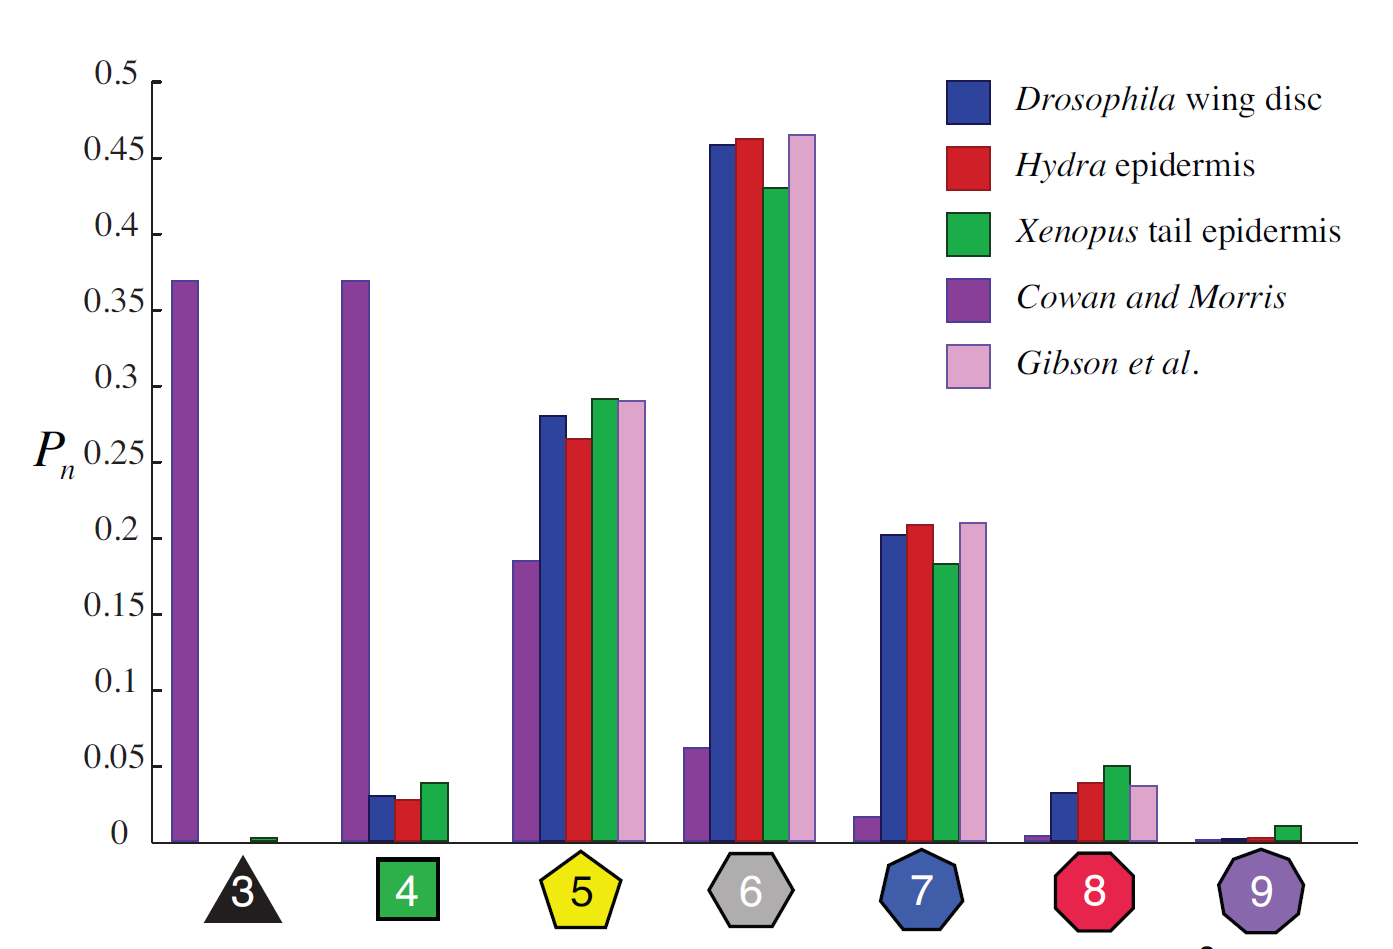
\includegraphics[height=5cm,width=5cm]{./tissueskinds.png}
    \end{column}
    \begin{column}{0.8\textwidth}
        \begin{itemize}
        \item Different cells \emph{shapes} distributions are related to \textbf{different kind} of tissues\footnotemark.
        \end{itemize}
    \end{column}
\end{columns}
\footcitetext{farhadifar2007influence}
\end{minipage}
\end{beamerboxesrounded}
}

%%tissue growth remarks
\frame{\frametitle{Developmental stages of tissues}
\setbeamercolor{uppercol}{fg=black,bg=pink}
\setbeamercolor{lowercol}{fg=black,bg=pink}
\begin{beamerboxesrounded}[upper=upperco,lower=lowercol,shadow=true]{}
\begin{minipage}[t]{6.1cm}
\begin{columns}
    \begin{column}{\textwidth}
        \hspace{0.4cm} 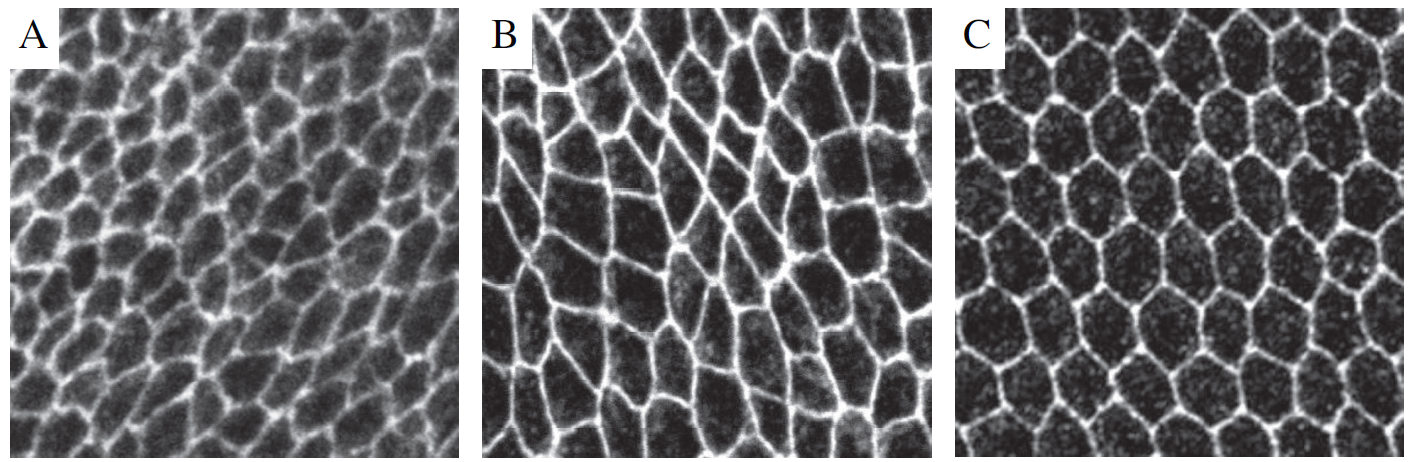
\includegraphics[height=5cm,width=5cm]{./devstages.png}
    \end{column}
    \begin{column}{0.8\textwidth}
        \begin{itemize}
        \item Different cells \emph{shapes} distributions are related to different \textbf{developmental stages} of a same tissue\footnotemark.
        \end{itemize}
    \end{column}
\end{columns}
\footcitetext{farhadifar2007influence}
\end{minipage}
\end{beamerboxesrounded}
}


\section{General Assumptions}
\subsection{General Assumptions}
%%tissue growth remarks
\frame{\frametitle{Tissue, cells, Edges, and Vertices}
\setbeamercolor{uppercol}{fg=black,bg=pink}
\setbeamercolor{lowercol}{fg=black,bg=pink}
\begin{beamerboxesrounded}[upper=upperco,lower=lowercol,shadow=true]{}
\begin{minipage}[t]{6.1cm}
\begin{columns}
    \begin{column}{\textwidth}
        \hspace{0.4cm} 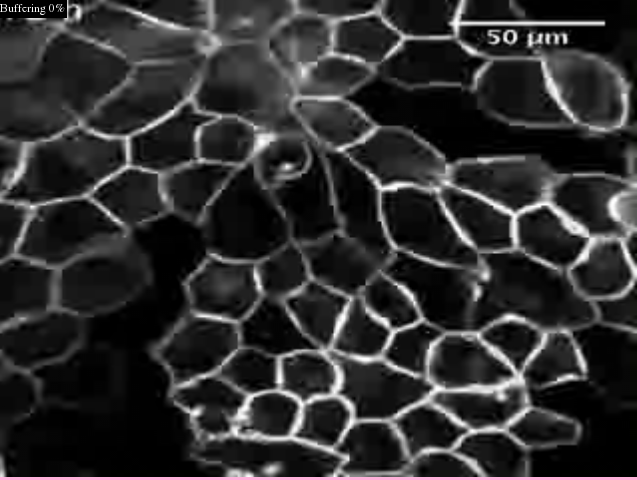
\includegraphics[height=5cm,width=5cm]{network_of_cells.png}
    \end{column}
    \begin{column}{0.8\textwidth}
        \begin{enumerate}
        \item < 1-| alert@1 > Tissue as a network of cells.
        \item < 2-| alert@2 > Cells as polygons.
        \item < 3-| alert@1 > Each 2 Cells share 1 Edge.
        \item < 4-| alert@2 > Each Edge is composed by 2 Vertices.
        \end{enumerate}
    \end{column}
\end{columns}
\footcitetext{farhadifar2007influence}
\end{minipage}
\end{beamerboxesrounded}
}


\subsection{Line Tension}
\frame{\frametitle{Edge's Line Tension}
\setbeamercolor{uppercol}{fg=black,bg=pink}
\setbeamercolor{lowercol}{fg=black,bg=pink}
\begin{beamerboxesrounded}[upper=upperco,lower=lowercol,shadow=true]{}
\begin{minipage}[t]{6.1cm}
\begin{columns}
    \begin{column}{\textwidth}
        \textbf{Include figure of a cell from Farhadifar}
    \end{column}
    \begin{column}{0.8\textwidth}
        \begin{itemize}
        \item Edge's Line tension ($\Lambda$) is associated to Edge's length.
        \end{itemize}
    \end{column}
\end{columns}
\end{minipage}
\end{beamerboxesrounded}
}


\subsection{Contractility}
\frame{\frametitle{Cell's Contractility}
\setbeamercolor{uppercol}{fg=black,bg=pink}
\setbeamercolor{lowercol}{fg=black,bg=pink}
\begin{beamerboxesrounded}[upper=upperco,lower=lowercol,shadow=true]{}
\begin{minipage}[t]{6.1cm}
\begin{columns}
    \begin{column}{\textwidth}
        \textbf{Include figure of a cell from Farhadifar}
    \end{column}
    \begin{column}{0.8\textwidth}
        \begin{itemize}
        \item Cell's Contractility ($\Gamma$) is associated to Cell's Perimeter.
        \end{itemize}
    \end{column}
\end{columns}
\end{minipage}
\end{beamerboxesrounded}
}

\subsection{Elasticity}
\frame{\frametitle{Cell's Elasticity}
\setbeamercolor{uppercol}{fg=black,bg=pink}
\setbeamercolor{lowercol}{fg=black,bg=pink}
\begin{beamerboxesrounded}[upper=upperco,lower=lowercol,shadow=true]{}
\begin{minipage}[t]{6.1cm}
\begin{columns}
    \begin{column}{\textwidth}
        \textbf{Include figure of a cell from Farhadifar}
    \end{column}
    \begin{column}{0.8\textwidth}
        \begin{itemize}
        \item Cell's Elasticity ($K$) is associated to Cell's Area.
        \end{itemize}
    \end{column}
\end{columns}
\end{minipage}
\end{beamerboxesrounded}
}

\subsection{Energy Function}
%%Minimal Energy
\frame{\frametitle{Force Balance Energy Function}
\setbeamercolor{uppercol}{fg=black,bg=pink}
\setbeamercolor{lowercol}{fg=black,bg=pink}
\begin{beamerboxesrounded}[upper=upperco,lower=lowercol,shadow=true]{}
\begin{minipage}[t]{6.1cm}
$F = \sum_{\alpha}{\frac{K_{\alpha}}{2}(A_{\alpha} - A_{\alpha}^{(0)})^{2} ~ + ~ \sum_{(i,j)}{\Lambda_{ij}L_{ij}} ~ + ~  \sum_{\alpha}{\frac{\Gamma_{\alpha}}{2}L_{\alpha}^{2}}}$
\end{minipage}
\end{beamerboxesrounded}
}

%%Minimal Energy
\frame{\frametitle{Force Balance Energy Function}
\setbeamercolor{uppercol}{fg=black,bg=pink}
\setbeamercolor{lowercol}{fg=black,bg=pink}
$F = \sum_{\alpha}{\frac{K_{\alpha}}{2}(A_{\alpha} - A_{\alpha}^{(0)})^{2} ~ + ~ \sum_{(i,j)}{\Lambda_{ij}L_{ij}} ~ + ~  \sum_{\alpha}{\frac{\Gamma_{\alpha}}{2}L_{\alpha}^{2}}}$
\begin{beamerboxesrounded}[upper=upperco,lower=lowercol,shadow=true]{}
\begin{minipage}[t]{6.1cm}
\begin{columns}
    \begin{column}{\textwidth}
       \hspace{0.4cm} 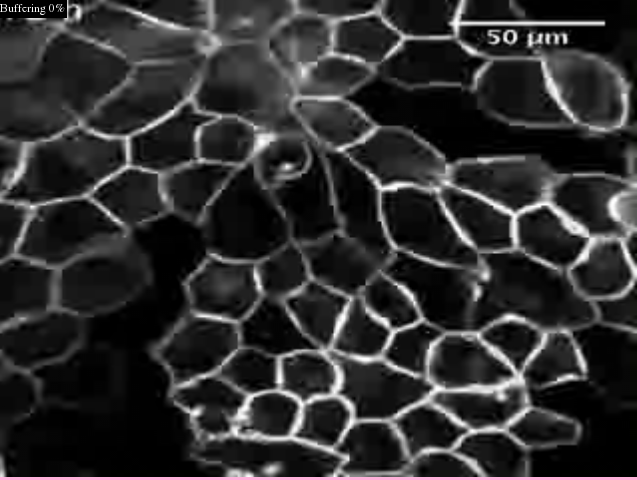
\includegraphics[height=5cm,width=5cm]{network_of_cells.png}
    \end{column}
    \begin{column}{0.8\textwidth}
       We keep the physical properties of the cells fixed during the simulation. So, in order to satisfy the \textbf{Minimal Energy's Assumption} theh positions of the vertices need to change.
    \end{column}
\end{columns}
\end{minipage}
\end{beamerboxesrounded}
}

%%Minimal Energy
\frame{\frametitle{Preferred Cell's Area $A_{\alpha}^{(0)}$}
\setbeamercolor{uppercol}{fg=black,bg=pink}
\setbeamercolor{lowercol}{fg=black,bg=pink}
$F = \sum_{\alpha}{\frac{K_{\alpha}}{2}(A_{\alpha} - A_{\alpha}^{(0)})^{2} ~ + ~ \sum_{(i,j)}{\Lambda_{ij}L_{ij}} ~ + ~  \sum_{\alpha}{\frac{\Gamma_{\alpha}}{2}L_{\alpha}^{2}}}$
\begin{beamerboxesrounded}[upper=upperco,lower=lowercol,shadow=true]{}
\begin{minipage}[t]{6.1cm}
\begin{columns}
    \begin{column}{\textwidth}
       \hspace{0.4cm} 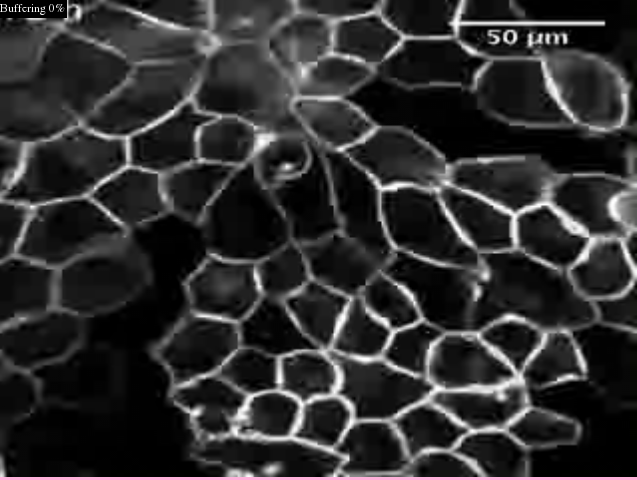
\includegraphics[height=5cm,width=5cm]{network_of_cells.png}
    \end{column}
    \begin{column}{0.8\textwidth}
    $A_{\alpha}^{(0)}$ is the preferred area of cell $\alpha$ which is related to the volume, $V_{\alpha}$ and height, $h_{\alpha}$ of the cell: $A_{\alpha}^{(0)} ~ = ~ \frac{V_{\alpha}}{h_{\alpha}} $
    \end{column}
\end{columns}
\end{minipage}
\end{beamerboxesrounded}
}


\section{Model Dynamics}
\subsection{Sequence of Events}
%%tissue growth remarks
\frame{\frametitle{Sequence of Events}
\setbeamercolor{uppercol}{fg=black,bg=pink}
\setbeamercolor{lowercol}{fg=black,bg=pink}
\begin{beamerboxesrounded}[upper=upperco,lower=lowercol,shadow=true]{}
\begin{minipage}[t]{6.1cm}
\begin{columns}
    \begin{column}{\textwidth}
        \hspace{4cm}\flashmovie[auto=0,loop=1,controlbar=1,engine=flv-player,width=6cm,height=6cm]{Animation.flv}
    \end{column}
    \begin{column}{0.8\textwidth}
        \begin{enumerate}
        \item < 1-| alert@1 > \textbf{Relaxation} (Vertices change their position to guarantee the force balance equal to zero).
        \item < 2-| alert@2 > \textbf{Cell Proliferation} (cells growth and cells division).
        \end{enumerate}
    \end{column}
\end{columns}
\end{minipage}
\end{beamerboxesrounded}
}


\subsection{Relaxation}
%%tissue growth remarks
\frame{\frametitle{Relaxation}
\setbeamercolor{uppercol}{fg=black,bg=pink}
\setbeamercolor{lowercol}{fg=black,bg=pink}
\begin{beamerboxesrounded}[upper=upperco,lower=lowercol,shadow=true]{}
\begin{minipage}[t]{6.1cm}
\begin{columns}
    \begin{column}{\textwidth}
        \hspace{1cm}\flashmovie[auto=0,loop=1,controlbar=1,engine=flv-player,width=6cm,height=6cm]{Animation.flv}
    \end{column}
    \begin{column}{0.8\textwidth}
        \begin{itemize}
        \item 1 - Vertices change their position to guarantee the force balance equal to zero.
        \end{itemize}
    \end{column}
\end{columns}
\end{minipage}
\end{beamerboxesrounded}
}


%%tissue growth remarks
\frame{\frametitle{Relaxation}
\setbeamercolor{uppercol}{fg=black,bg=pink}
\setbeamercolor{lowercol}{fg=black,bg=pink}
\begin{beamerboxesrounded}[upper=upperco,lower=lowercol,shadow=true]{}
\begin{minipage}[t]{6.1cm}
\begin{columns}
    \begin{column}{\textwidth}
        \hspace{1cm}\flashmovie[auto=0,loop=1,controlbar=1,engine=flv-player,width=6cm,height=6cm]{Animation.flv}
    \end{column}
    \begin{column}{0.8\textwidth}
        \begin{itemize}
        \item 2 - The position of the vertices is defined by a \emph{Verlet Function}\cite{Farhadifar} in which the accelleration is defined by the total force on the junctions of the tissue ($r(t ~ + ~ \Delta t) = ~ 2r(t) ~ - ~ r(t ~ - ~ \Delta t) + a(t)\Delta t^{2} $).
        \end{itemize}
    \end{column}
\end{columns}
\end{minipage}
\end{beamerboxesrounded}
}


%%tissue growth remarks
\frame{\frametitle{Relaxation}
\setbeamercolor{uppercol}{fg=black,bg=pink}
\setbeamercolor{lowercol}{fg=black,bg=pink}
\begin{beamerboxesrounded}[upper=upperco,lower=lowercol,shadow=true]{}
\begin{minipage}[t]{6.1cm}
\begin{columns}
    \begin{column}{\textwidth}
        \hspace{1cm}\flashmovie[auto=0,loop=1,controlbar=1,engine=flv-player,width=6cm,height=6cm]{Animation.flv}
    \end{column}
    \begin{column}{0.8\textwidth}
        \begin{itemize}
        \item 3 - Once the force is zero, the accelleration of the \emph{Verlet Function} is also zero, and so the position of the vertices don't change from time step $t$ to $t + \Delta t$. 
        \end{itemize}
    \end{column}
\end{columns}
\end{minipage}
\end{beamerboxesrounded}
}

%%tissue growth remarks
\frame{\frametitle{Relaxation}
\setbeamercolor{uppercol}{fg=black,bg=pink}
\setbeamercolor{lowercol}{fg=black,bg=pink}
\begin{beamerboxesrounded}[upper=upperco,lower=lowercol,shadow=true]{}
\begin{minipage}[t]{6.1cm}
\begin{columns}
    \begin{column}{\textwidth}
        \hspace{1cm}\flashmovie[auto=0,loop=1,controlbar=1,engine=flv-player,width=6cm,height=6cm]{Animation.flv}
    \end{column}
    \begin{column}{0.8\textwidth}
        \begin{itemize}
        \item 4 - Relaxation is finished once the length of the tissue remains \emph{steady} (the position of its vertices don't change) along 100 time steps ($\frac{sd(\sum_{\alpha}{L_{\alpha}})}{mean({\sum_{\alpha}{L_{\alpha}}})} \apeq 0 $).
        \end{itemize}
    \end{column}
\end{columns}
\end{minipage}
\end{beamerboxesrounded}
}


%%tissue growth remarks
\frame{\frametitle{\emph{Regularness of the tissue}}
\setbeamercolor{uppercol}{fg=black,bg=pink}
\setbeamercolor{lowercol}{fg=black,bg=pink}
\begin{beamerboxesrounded}[upper=upperco,lower=lowercol,shadow=true]{}
\begin{minipage}[t]{6.1cm}
    \begin{enumerate}
    \item < 1-| alert@1 > We define \textbf{\emph{regularness}} as a dimensionless measure to say how regular the cells of a tissue are.
    \item < 2-| alert@1 > Regularness is defined as: $Reg = \frac{sd(L_{ij})}{mean(L_{ij})}$ over all the edges.
    \end{enumerate}
\end{minipage}
\end{beamerboxesrounded}
}


%%tissue growth remarks
\frame{\frametitle{\emph{Regularness of the tissue}}
\setbeamercolor{uppercol}{fg=black,bg=pink}
\setbeamercolor{lowercol}{fg=black,bg=pink}
We define \textbf{\emph{regularness}} as a dimensionless measure to say how regular the cells of a tissue are.
\begin{beamerboxesrounded}[upper=upperco,lower=lowercol,shadow=true]{}
\begin{minipage}[t]{6.1cm}
\begin{columns}
    \begin{column}{\textwidth}
        \begin{center}
            $Reg ~ \apeq ~ 0$
        \end{center}
        \hspace{0.4cm} 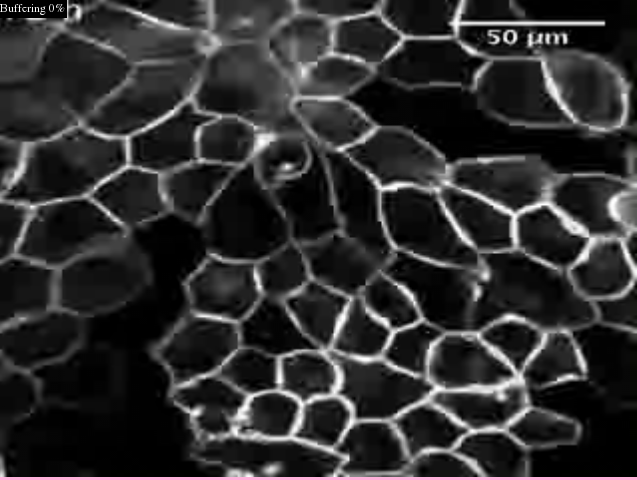
\includegraphics[height=4cm,width=4cm]{network_of_cells.png}
    \end{column}
    \begin{column}{\textwidth}
        \begin{center}
            $Reg ~ > ~ 0$
        \end{center}
        \hspace{0.4cm} 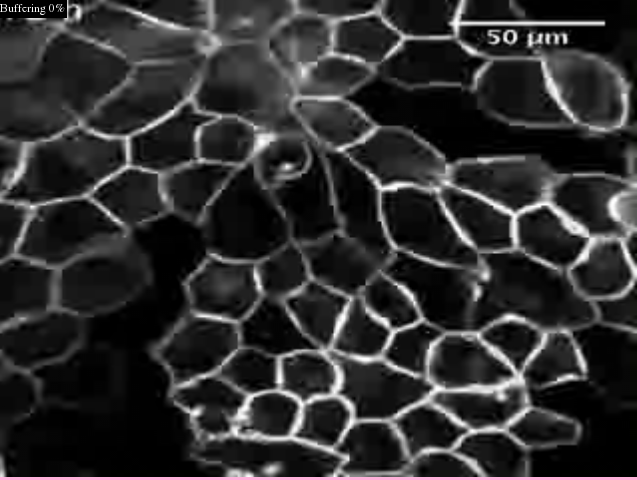
\includegraphics[height=4cm,width=4cm]{network_of_cells.png}
    \end{column}
\end{columns}
\end{minipage}
\end{beamerboxesrounded}
}


%%tissue growth remarks
\frame{\frametitle{\emph{Phase space of Regularness}}
\setbeamercolor{uppercol}{fg=black,bg=pink}
\setbeamercolor{lowercol}{fg=black,bg=pink}
\begin{beamerboxesrounded}[upper=upperco,lower=lowercol,shadow=true]{}
\begin{minipage}[t]{6.1cm}
\centering 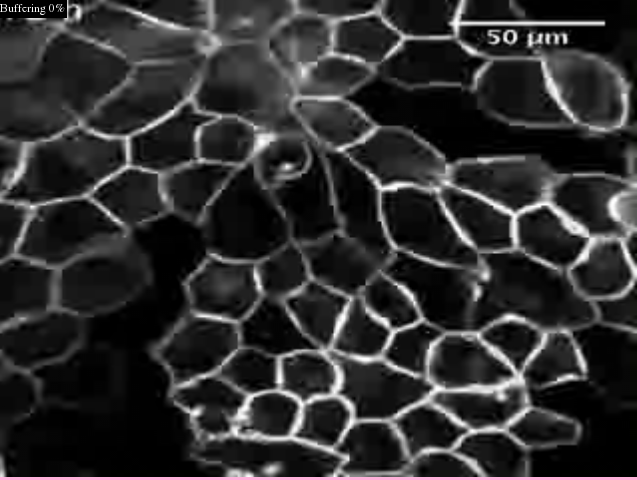
\includegraphics[height=4cm,width=4cm]{network_of_cells.png}
\end{minipage}
\end{beamerboxesrounded}
}


%%tissue growth remarks
\frame{\frametitle{\emph{Phase space of Regularness in Time}}
\setbeamercolor{uppercol}{fg=black,bg=pink}
\setbeamercolor{lowercol}{fg=black,bg=pink}
\begin{beamerboxesrounded}[upper=upperco,lower=lowercol,shadow=true]{}
\begin{minipage}[t]{6.1cm}
\centering \flashmovie[auto=0,loop=1,controlbar=1,engine=flv-player,width=6cm,height=6cm]{Animation.flv}
\end{minipage}
\end{beamerboxesrounded}
}



%%%%%%%% CELL DIVISION

\subsection{Cell Proliferation}
%%tissue growth remarks
\frame{\frametitle{Cell Proliferation}
\setbeamercolor{uppercol}{fg=black,bg=pink}
\setbeamercolor{lowercol}{fg=black,bg=pink}
\begin{beamerboxesrounded}[upper=upperco,lower=lowercol,shadow=true]{}
\begin{minipage}[t]{6.1cm}
\begin{columns}
    \begin{column}{\textwidth}
        \hspace{1cm}\flashmovie[auto=0,loop=1,controlbar=1,engine=flv-player,width=6cm,height=6cm]{Animation.flv}
    \end{column}
    \begin{column}{0.8\textwidth}
        \begin{itemize}
        \item Cell Growth.
        \item Cell Division.
        \end{itemize}
    \end{column}
\end{columns}
\end{minipage}
\end{beamerboxesrounded}
}


\subsection{Cell Growth}
%%tissue growth remarks
\frame{\frametitle{Cell Growth}
\setbeamercolor{uppercol}{fg=black,bg=pink}
\setbeamercolor{lowercol}{fg=black,bg=pink}
\begin{beamerboxesrounded}[upper=upperco,lower=lowercol,shadow=true]{}
\begin{minipage}[t]{6.1cm}
\begin{columns}
    \begin{column}{\textwidth}
        \hspace{1cm}\flashmovie[auto=0,loop=1,controlbar=1,engine=flv-player,width=6cm,height=6cm]{Animation.flv}
    \end{column}
    \begin{column}{0.8\textwidth}
        \begin{enumerate}
        \item < 1-| alert@1 > Cells are \textbf{randomly} triggered to increase their area.
        \item < 2-| alert@2 > They increase their area by 10\% each time step.
        \end{enumerate}
    \end{column}
\end{columns}
\end{minipage}
\end{beamerboxesrounded}
}

%%tissue growth remarks
\frame{\frametitle{Cell Growth}
\setbeamercolor{uppercol}{fg=black,bg=pink}
\setbeamercolor{lowercol}{fg=black,bg=pink}
$F = \sum_{\alpha}{\frac{K_{\alpha}}{2}(A_{\alpha} - A_{\alpha}^{(0)})^{2} ~ + ~ \sum_{(i,j)}{\Lambda_{ij}L_{ij}} ~ + ~  \sum_{\alpha}{\frac{\Gamma_{\alpha}}{2}L_{\alpha}^{2}}}$
\begin{beamerboxesrounded}[upper=upperco,lower=lowercol,shadow=true]{}
\begin{minipage}[t]{6.1cm}
\begin{columns}
    \begin{column}{\textwidth}
        \hspace{1cm}\flashmovie[auto=0,loop=1,controlbar=1,engine=flv-player,width=6cm,height=6cm]{Animation.flv}
    \end{column}
    \begin{column}{0.8\textwidth}
        \begin{enumerate}
        \item < 1-| alert@1 > The increment of the area is given by changing the value of the preferred area parameter ($A_{\alpha}^{(0)}$) on the Force balance equation.
        \end{enumerate}
    \end{column}
\end{columns}
\end{minipage}
\end{beamerboxesrounded}
}

\subsection{Cell Division}
%%tissue growth remarks
\frame{\frametitle{Cell Division}
\setbeamercolor{uppercol}{fg=black,bg=pink}
\setbeamercolor{lowercol}{fg=black,bg=pink}
$F = \sum_{\alpha}{\frac{K_{\alpha}}{2}(A_{\alpha} - A_{\alpha}^{(0)})^{2} ~ + ~ \sum_{(i,j)}{\Lambda_{ij}L_{ij}} ~ + ~  \sum_{\alpha}{\frac{\Gamma_{\alpha}}{2}L_{\alpha}^{2}}}$
\begin{beamerboxesrounded}[upper=upperco,lower=lowercol,shadow=true]{}
\begin{minipage}[t]{6.1cm}
\begin{columns}
    \begin{column}{\textwidth}
        \hspace{1cm}\flashmovie[auto=0,loop=1,controlbar=1,engine=flv-player,width=6cm,height=6cm]{Animation.flv}
    \end{column}
    \begin{column}{0.8\textwidth}
        \begin{enumerate}
        \item < 1-| alert@1 > Once a cell $\alpha$ reaches the \textbf{double} of the area it had \textbf{before starting to increase}, it is subdivided into two cells with half the current area of cell $\alpha$.
        \end{enumerate}
    \end{column}
\end{columns}
\end{minipage}
\end{beamerboxesrounded}
}

%%tissue growth remarks
\frame{\frametitle{Cell Division}
\setbeamercolor{uppercol}{fg=black,bg=pink}
\setbeamercolor{lowercol}{fg=black,bg=pink}
$F = \sum_{\alpha}{\frac{K_{\alpha}}{2}(A_{\alpha} - A_{\alpha}^{(0)})^{2} ~ + ~ \sum_{(i,j)}{\Lambda_{ij}L_{ij}} ~ + ~  \sum_{\alpha}{\frac{\Gamma_{\alpha}}{2}L_{\alpha}^{2}}}$
\begin{beamerboxesrounded}[upper=upperco,lower=lowercol,shadow=true]{}
\begin{minipage}[t]{6.1cm}
\begin{columns}
    \begin{column}{\textwidth}
        \hspace{1cm}\flashmovie[auto=0,loop=1,controlbar=1,engine=flv-player,width=6cm,height=6cm]{Animation.flv}
    \end{column}
    \begin{column}{0.8\textwidth}
        \begin{enumerate}
        \item < 1-| alert@1 > The division consists in creating a new edge $e_{i}$ that \textbf{crosses the centroid} of the original cell $\alpha$ with a \textbf{random direction}.
        \end{enumerate}
    \end{column}
\end{columns}
\end{minipage}
\end{beamerboxesrounded}
}


%%tissue growth remarks
\frame{\frametitle{Cell Division}
\setbeamercolor{uppercol}{fg=black,bg=pink}
\setbeamercolor{lowercol}{fg=black,bg=pink}
$F = \sum_{\alpha}{\frac{K_{\alpha}}{2}(A_{\alpha} - A_{\alpha}^{(0)})^{2} ~ + ~ \sum_{(i,j)}{\Lambda_{ij}L_{ij}} ~ + ~  \sum_{\alpha}{\frac{\Gamma_{\alpha}}{2}L_{\alpha}^{2}}}$
\begin{beamerboxesrounded}[upper=upperco,lower=lowercol,shadow=true]{}
\begin{minipage}[t]{6.1cm}
\begin{columns}
    \begin{column}{\textwidth}
        \hspace{1cm}\flashmovie[auto=0,loop=1,controlbar=1,engine=flv-player,width=6cm,height=6cm]{Animation.flv}
    \end{column}
    \begin{column}{0.8\textwidth}
        \begin{enumerate}
        \item < 1-| alert@1 > The former cell $\alpha$ is replaced by two new cells that share the edge $e_{i}$.
        \end{enumerate}
    \end{column}
\end{columns}
\end{minipage}
\end{beamerboxesrounded}
}


%%tissue growth remarks
\frame{\frametitle{Cell Division}
\setbeamercolor{uppercol}{fg=black,bg=pink}
\setbeamercolor{lowercol}{fg=black,bg=pink}
$F = \sum_{\alpha}{\frac{K_{\alpha}}{2}(A_{\alpha} - A_{\alpha}^{(0)})^{2} ~ + ~ \sum_{(i,j)}{\Lambda_{ij}L_{ij}} ~ + ~  \sum_{\alpha}{\frac{\Gamma_{\alpha}}{2}L_{\alpha}^{2}}}$
\begin{beamerboxesrounded}[upper=upperco,lower=lowercol,shadow=true]{}
\begin{minipage}[t]{6.1cm}
\begin{columns}
    \begin{column}{\textwidth}
        \hspace{1cm}\flashmovie[auto=0,loop=1,controlbar=1,engine=flv-player,width=6cm,height=6cm]{Animation.flv}
    \end{column}
    \begin{column}{0.8\textwidth}
        \begin{enumerate}
        \item < 1-| alert@1 > Edges in neighbour cells that are now connected to one of the vertices of $e_{i}$ need to be splitted into two edges.
        \end{enumerate}
    \end{column}
\end{columns}
\end{minipage}
\end{beamerboxesrounded}
}


%%tissue growth remarks
\frame{\frametitle{Cell Division}
\setbeamercolor{uppercol}{fg=black,bg=pink}
\setbeamercolor{lowercol}{fg=black,bg=pink}
$F = \sum_{\alpha}{\frac{K_{\alpha}}{2}(A_{\alpha} - A_{\alpha}^{(0)})^{2} ~ + ~ \sum_{(i,j)}{\Lambda_{ij}L_{ij}} ~ + ~  \sum_{\alpha}{\frac{\Gamma_{\alpha}}{2}L_{\alpha}^{2}}}$
\begin{beamerboxesrounded}[upper=upperco,lower=lowercol,shadow=true]{}
\begin{minipage}[t]{6.1cm}
\begin{columns}
    \begin{column}{\textwidth}
        \hspace{1cm}\flashmovie[auto=0,loop=1,controlbar=1,engine=flv-player,width=6cm,height=6cm]{Animation.flv}
    \end{column}
    \begin{column}{0.8\textwidth}
        \begin{enumerate}
        \item < 1-| alert@1 > This procedure changes the \emph{shape} of the cells in the neighbourhood of $\alpha$, as well as it creates new cells to replace $\alpha$ that not necessarily have the same \emph{shape} as $\alpha$.
        \end{enumerate}
    \end{column}
\end{columns}
\end{minipage}
\end{beamerboxesrounded}
}


\subsection{Steady State}
%%tissue growth remarks
\frame{\frametitle{Steady state}
\setbeamercolor{uppercol}{fg=black,bg=pink}
\setbeamercolor{lowercol}{fg=black,bg=pink}
$F = \sum_{\alpha}{\frac{K_{\alpha}}{2}(A_{\alpha} - A_{\alpha}^{(0)})^{2} ~ + ~ \sum_{(i,j)}{\Lambda_{ij}L_{ij}} ~ + ~  \sum_{\alpha}{\frac{\Gamma_{\alpha}}{2}L_{\alpha}^{2}}}$
\begin{beamerboxesrounded}[upper=upperco,lower=lowercol,shadow=true]{}
\begin{minipage}[t]{6.1cm}
\begin{columns}
    \begin{column}{\textwidth}
        \hspace{0.4cm} 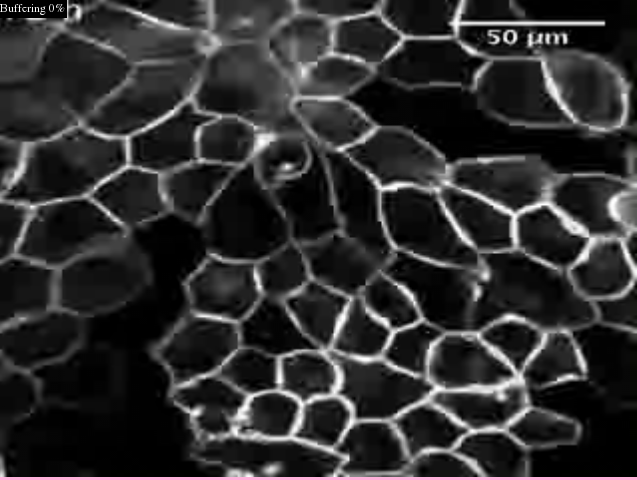
\includegraphics[height=4cm,width=4cm]{network_of_cells.png}
    \end{column}
    \begin{column}{0.8\textwidth}
        \begin{enumerate}
        \item < 1-| alert@1 > The steady state of the cell division proccess is observed once the relative proportion of cells don't change along 1000 time steps.
        \end{enumerate}
    \end{column}
\end{columns}
\end{minipage}
\end{beamerboxesrounded}
}

\section{Results}
\subsection{Results}
%%tissue growth remarks
\frame{\frametitle{Phase Space: Mean shape of cells}
\setbeamercolor{uppercol}{fg=black,bg=pink}
\setbeamercolor{lowercol}{fg=black,bg=pink}
$F = \sum_{\alpha}{\frac{K_{\alpha}}{2}(A_{\alpha} - A_{\alpha}^{(0)})^{2} ~ + ~ \sum_{(i,j)}{\Lambda_{ij}L_{ij}} ~ + ~  \sum_{\alpha}{\frac{\Gamma_{\alpha}}{2}L_{\alpha}^{2}}}$
\begin{beamerboxesrounded}[upper=upperco,lower=lowercol,shadow=true]{}
\begin{minipage}[t]{6.1cm}
\begin{columns}
    \begin{column}{\textwidth}
        \hspace{0.4cm} 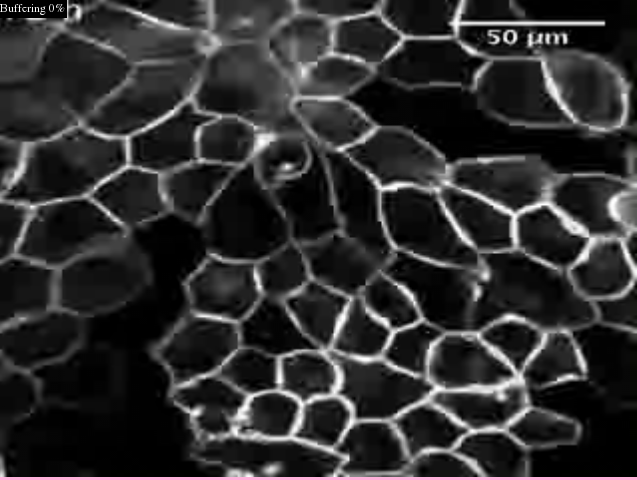
\includegraphics[height=4cm,width=4cm]{network_of_cells.png}
    \end{column}
    \begin{column}{0.8\textwidth}
        \begin{enumerate}
        \item < 1-| alert@1 > We observed the following Phase space of shape of cells after 10 replicates.
        \end{enumerate}
    \end{column}
\end{columns}
\end{minipage}
\end{beamerboxesrounded}
}

\frame{\frametitle{Phase Space: Deviation of shapes of cells}
\setbeamercolor{uppercol}{fg=black,bg=pink}
\setbeamercolor{lowercol}{fg=black,bg=pink}
$F = \sum_{\alpha}{\frac{K_{\alpha}}{2}(A_{\alpha} - A_{\alpha}^{(0)})^{2} ~ + ~ \sum_{(i,j)}{\Lambda_{ij}L_{ij}} ~ + ~  \sum_{\alpha}{\frac{\Gamma_{\alpha}}{2}L_{\alpha}^{2}}}$
\begin{beamerboxesrounded}[upper=upperco,lower=lowercol,shadow=true]{}
\begin{minipage}[t]{6.1cm}
\begin{columns}
    \begin{column}{\textwidth}
        \hspace{0.4cm} 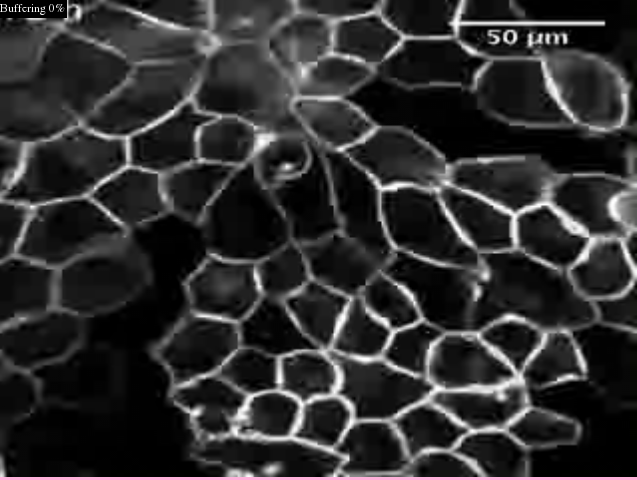
\includegraphics[height=4cm,width=4cm]{network_of_cells.png}
    \end{column}
    \begin{column}{0.8\textwidth}
        \begin{enumerate}
        \item < 1-| alert@1 > We observed the following Phase space of the variation in the shape of cells after 10 replicates.
        \end{enumerate}
    \end{column}
\end{columns}
\end{minipage}
\end{beamerboxesrounded}
}


\section{Next Steps}
\subsection{Next Steps}
%%tissue growth remarks
\frame{\frametitle{Phase Space: Mean shape of cells}
\setbeamercolor{uppercol}{fg=black,bg=pink}
\setbeamercolor{lowercol}{fg=black,bg=pink}
$F = \sum_{\alpha}{\frac{K_{\alpha}}{2}(A_{\alpha} - A_{\alpha}^{(0)})^{2} ~ + ~ \sum_{(i,j)}{\Lambda_{ij}L_{ij}} ~ + ~  \sum_{\alpha}{\frac{\Gamma_{\alpha}}{2}L_{\alpha}^{2}}}$
\begin{beamerboxesrounded}[upper=upperco,lower=lowercol,shadow=true]{}
\begin{minipage}[t]{6.1cm}
    \begin{enumerate}
    \item < 1-| alert@1 > Increase the number of replicates.
    \item < 2-| alert@2 > Change initial conditions of the tissues.
    \item < 3-| alert@3 > Change choice of cells to proliferate.
    \item < 4-| alert@4 > Change the way cells are divided.
    \item < 5-| alert@5 > Change the shape of the tissue.
    \end{enumerate}
\end{minipage}
\end{beamerboxesrounded}
}


\section{Acknowledgments}
\frame{\frametitle{Thank you!}
\begin{itemize}
\item SystemsX Initiative.
\item \textbf{\emph{EpiphysX}} members: Andreas Wagner (UZH), Aziza Merzouki, Orestis Malaspinas, Bastien Chopard, Aur\'elien Roux, Michel Milinkovitch, Marcos Gonzalez-Gaitan (UNIGE) 
\item Chopard's Group members (UNIGE).
\item Wagner's Group members (UZH).
\item You, for the attention and patience.
\end{itemize}
}
%%%%%%%%%%%%%%%%%%%%%%%%%%%%%%%%%%%%%%%%%%%%%%%%%%%%%%%%%%%%%%%%%%%%%%%%%%%%%%%%%%%%%%%%%%
%%%%%%%%%%%%%%%%%%%%%%%%%%%%%% End Document %%%%%%%%%%%%%%%%%%%%%%%%%%%%%%%%%%%%%%%%%%%%%%
%%%%%%%%%%%%%%%%%%%%%%%%%%%%%%%%%%%%%%%%%%%%%%%%%%%%%%%%%%%%%%%%%%%%%%%%%%%%%%%%%%%%%%%%%%
\end{document}


